\documentclass[main.tex]{subfiles}
\begin{document}



\section{Metrieken op functieruimten}
\label{sec:metr-op-funct}

\begin{de}
  Zij $X$ een gesloten, begrensd deel van $\mathbb{R}^{p}$. Dan noteren we met $C(X)$ de vectorruimte van de continue functies van $X$ naar $\mathbb{R}$.
\end{de}

\begin{de}
  Zij $\interval{a}{b}$ een gesloten, begrensd interval in $\mathbb{R}$, dan noteren we met $C(\interval{a}{b})$ de vectorruimte van de continue functies van $\interval{a}{b}$ naar $\mathbb{R}$.
\end{de}

\subsection{De supremum metriek}
\label{sec:supremum-metriek}

\begin{vb}
  Zij $X$ een gesloten en begrensde deelverzameling van $\mathbb{R}^{p}$, dan is $C(X)$, uitgerust met de volgende functie als metriek, een metrische ruimte:
  \[ d_{\infty}:\ C(x)\times C(X)\rightarrow \mathbb{R}^{+}:\ (f,g) \mapsto d_{\infty}(f,g) = \sup \{ |f(x)-g(x)| \mid x \in X \} \]

  \extra{bewijs}
\end{vb}

\begin{opm}
  Merk op dat dit goed gedefinieerd is omdat $|f(x)-g(x)|$ voor continue functies op een gesloten, begrensd deel steeds begrensd blijft. \needed
\end{opm}

\begin{vb}
  Een open bol $B(f,\delta)$ in $C(\interval{a}{b})$ ziet er als volgt uit:
  \[ B(f,\delta) = \{ g \in C(\interval{a}{b} \mid  \forall x\in \interval{a}{b}:\ |g(x)-f(x)|< \delta \} \]
  \begin{figure}[H]
    \centering
    \begin{tikzpicture}[scale=.75]
      \begin{axis}[ymin=-0.5, ymax=4, xmin=-2.9, xmax=2.9, no markers]
        \addplot[smooth,color=red,thick,domain=-3:-1]{-x};
        \addplot[smooth,color=red,thick,domain=-1:1]{x^2};
        \addplot[smooth,color=red,thick,domain=1:3]{x^3};
        \addplot[name path=A,smooth,color=black!20,thick,domain=-3:-1]{-x+0.25};
        \addplot[name path=B,smooth,color=black!20,thick,domain=-3:-1]{-x-0.25};
        \addplot[black!20] fill between[of=A and B];
        \addplot[name path=A,smooth,color=black!20,thick,domain=-1:1]{x^2+0.25};
        \addplot[name path=B,smooth,color=black!20,thick,domain=-1:1]{x^2-0.25};
        \addplot[black!20] fill between[of=A and B];
        \addplot[name path=A,smooth,color=black!20,thick,domain=1:3]{x^3+0.25};
        \addplot[name path=B,smooth,color=black!20,thick,domain=1:3]{x^3-0.25};
        \addplot[black!20] fill between[of=A and B];
      \end{axis}
    \end{tikzpicture}
    \caption{ Een illustratie van een open bol in $C(\interval{3}{3})$ rond een functie voor $p=1$. }
  \end{figure}

  \noindent
  Merk op dat dit slechts een illustratie is.
  Elke functie die volledig binnen de $\delta$-strook ligt, ligt binnen de open bol.
  Merk ook op dat de strook overal even breed is, ookal lijkt ze smaller voor een sterker stijgend deel van de functie.
\end{vb}

\begin{vb}
  Zij $f_{1},f_{2}:\ \interval{0}{1} \rightarrow \mathbb{R}$ twee continue functies met de volgende eigenschap
  \[ \forall t\in \interval{0}{1}:\ f_{1}(t) < f_{2}(t) \]
  Benoem een deelverzameling $A$ van $C(\interval{0}{1})$ als volgt:
  \[ A = \{ f\in C(\interval{0}{1}) \mid \forall t\in \interval{0}{1}:\ f_{1}(t) < f(t) < f_{2}(t) \} \]
  $A$ is dan $d_{\infty}$ open.

  \begin{proof}
    Kies een willekeurige $f\in A$.
    Voor alle $t\in \interval{0}{1}$ is $f(t) - f_{1}(t)$ strikt positief.
    Omdat $f-f_{1}$ continu is\prref{pr:optelling-continu} en $\interval{0}{1}$ gesloten\stref{st:gesloten-interval-gesloten} en begrensd, bestaat er een $r_{1}\in\mathbb{R}_{0}^{+}$ zodat $\forall t\in \interval{0}{1}:\ f(t)-f_{1}(t) > r_{1}$ geldt.
    Analoog bestaat er een $r_{2}\in \mathbb{R}^{+}$ zodat $\forall t\in \interval{0}{1}:\ f_{2}(t) -f(t) > r_{2}$
    Noem nu $r=\min\{r_{1},r_{2}\}$ en kies een willekeurige $g\in B_{\infty}(f,r)$, dan geldt het volgende en zit $g$ dus in $A$.
    \[ \forall t\in \interval{0}{1}:\ f_{1}(t) < f(t) - r_{1} \le f(t) - r < g(t) < f(t) + r \le f(t) + r_{2} < f_{2}(t) \]

    \begin{figure}[H]
      \centering
      \begin{tikzpicture}
        \begin{axis}[ymin=-1.1, ymax=1.1, xmin=-0.1, xmax=1.1, no markers]
          \addplot[name path=A,smooth,color=red,ultra thick,domain=0:1]{sin(150*x+60)};
          \addplot[name path=B,smooth,color=red,ultra thick,domain=0:1]{cos(150*x+60)};
          \addplot[black!20] fill between[of=A and B];

          \addplot[smooth,domain=0:1]{-1.45*x^2+0.75};
          \addplot[name path=C,smooth,color=black!30,thick,domain=0:1]{-1.5*x^2+0.75+0.1};
          \addplot[name path=D,smooth,color=black!30,thick,domain=0:1]{-1.5*x^2+0.75-0.1};
          \addplot[black!40] fill between[of=C and D];
        \end{axis}
      \end{tikzpicture}
      \caption{ Een illustratie van de situatie voor twee gekozen functies (rood), een willekeurige functie in $A$ (zwart) en een strook er rond om een open bol voor te stellen.}
    \end{figure}
  \end{proof}
\end{vb}


\begin{st}
  Een rij $(f_{n})_{n}$ in $C(X)$ zal volgens de $d_{\infty}$ metriek convergeren naar een $f\in C(X)$ als en slechts als $(f_{n})_{n}$ uniform naar $f$ convergeert.

\extra{bewijs: ookal is het al duidelijk}
Hint uit les: zie forum, Eline heeft dit uitgeschreven.
Let wel op de ongelijheid met het supremum.
\end{st}

\begin{vb}
  Beschouw de functie $I$ als volgt:
  \[ I:\ C(\interval{a}{b}) \rightarrow \mathbb{R}:\ f \mapsto \int_{a}^{b}f(x)\ dx \]
  $I$ is continu als we op $C(\interval{a}{b})$ de $d_{\infty}$-metriek beschouwen en op $\mathbb{R}$ de gewone metriek.
\extra{bewijs}
\end{vb}

\begin{vb}
  Beschouw de deelverzameling $N$, als volgt, van $C(\interval{0}{1})$.
  \[ N = \{ f \in C(\interval{0}{1}) \mid f(0) = 0 \} \]
  Voor $d_{\infty}$ is $\mathring{N}$ is dan leeg en $\overline{N}$ is heel $N$.

  \begin{proof}
    \noindent
    \begin{itemize}
    \item Kies willekeurig een $f\in N$ en willekeurig een $\epsilon \in \mathbb{R}_{0}^{+}$.
      Beschouw de functie $g=f+\frac{\epsilon}{2}$.
      $g$ zit dan in $C(\interval{0}{1})\setminus N$ en ligt op een afstand kleiner dan $\epsilon$ van $f$, maar zit niet in $N$.
    \item De sluiting van $N$ is $N$ zelf want $N$ is $d_{\infty}$-gesloten.
      Kies immers een rij $(f_{n})_{n}$ in $N$ die puntsgewijs (?!) naar een $f\in C(\interval{0}{1})$ convergeert.
      Omdat $\forall n\in \mathbb{N}:\ |f_{n}(0)-f(0)| \le d_{\infty}(f_{n},f)$ geldt en $(f_{n})_{n}$ naar $f$ convergeert zal $(f_{n}(0))_{n}$ naar $f(0)$ convergeren.
      Omdat $f_{n}(0)$ steeds nul is zal dus ook $f(0)$ nul zijn en $f$ dus in $N$ zitten.
    \end{itemize}
  \end{proof}
\end{vb}

\begin{vb}
  Beschouw de verzameling van positieve functies $A$ als volgt:
  \[ A = \{ f \in C(\interval{0}{1}) \mid \forall t\in \interval{0}{1}:\ f(t) \ge 0 \} \]
  $A$ is gesloten (dus $\overline{A}=A$) en $\mathring{A}$ ziet er als volgt uit:
  \[ \mathring{A} = \{ f \in C(\interval{0}{1}) \mid \forall t\in \interval{0}{1}:\ f(t) > 0 \} \]
  De rand $\partial A$ ziet er dus als volgt uit:
  \[ \partial A = \{ f \in C(\interval{0}{1}) \mid \forall t\in \interval{0}{1}:\ f(t) \ge 0 \wedge \exists t \in \interval{0}{1}:\ f(t) = 0 \} \]
  $A$ bevat bovendien enkel ophopingspunten en heeft geen ge\"isoleerde punten.

\extra{bewijs}
\end{vb}

\begin{vb}
  De verzamelingen $C\left(\interval{0}{1}\right)$, $C\left(\interval{a}{b}\right)$, $C_{0}\left(\mathbb{R}\right)$ en $C_{b}\left(\mathbb{R}\right)$, zijn separabel.
\TODO{bewijs}
\end{vb}

\begin{opm}
  Als dit niet het geval was, dan was numerieke modellering niet nuttig.
\end{opm}

\begin{vb}
  De ruimte $X$ van continue functies van $\interval{0}{1} \cup \interval{2}{3}$ naar $\mathbb{R}$, uitgerust met de supremummetriek is samenhangend.

  \begin{proof}
    Merk eerst op dat $d_{\infty}$ een norm induceert op $X$:\deref{norm}
    \[ |f|_{\infty} = d(f_{\infty},0) \]
    $X$ is bovendien een convexe verzameling en daarom samenhangend.\prref{pr:convexe-deelverzamelingen-samenhangend}
  \end{proof}
\end{vb}


\subsection{De $d_1$-metriek op $C(\interval{0}{1})$}
\label{sec:de-d_1-metriek}

\begin{vb}
  Zij $\interval{a}{b}$ een gesloten en begrensd interval, dan is $C(\interval{a}{b})$,, uitgerust met de volgende functie als metriek, een metrische ruimte:
  \[ d_{1}:\ C(\interval{a}{b})\times C(\interval{a}{b}) \rightarrow \mathbb{R}^{+}:\ (f,g) \mapsto \int_{a}^{b}|f(x)-g(x)|dx \]
\extra{bewijs}
\end{vb}

\begin{opm}
  In deze metrische ruimte is het moeilijk om open bollen te tekenen, het inwendige van een deel van $C(\interval{a}{b})$ is namelijk steeds leeg.
\end{opm}


\begin{vb}
  Beschouw de rij functies $(f_{n})_{n}$ in $C(\interval{0}{1})$ gegeven als volgt:

  \noindent
  \begin{minipage}{.45\textwidth}
    \begin{figure}[H]
      \centering
      \begin{tikzpicture}[scale=.75]
        \begin{axis}[ymin=-1.1, ymax=1.1, xmin=-0.1, xmax=1.1]
          \foreach \i in {1,...,10}
          {
            \addplot[smooth,domain=0:(1/(2*\i))]{2*\i*x};
            \addplot[smooth,domain=(1/(2*\i)):(1/\i)]{2-2*\i*x};
            \addplot[smooth,domain=(1/(\i)):1.1]{0};
          }
          \addplot[smooth,color=red,ultra thick,domain=-3:3]{0};
          \addplot[soldot,color=red] coordinates {(0,0)};
        \end{axis}
      \end{tikzpicture}
    \end{figure}
  \end{minipage}
  \begin{minipage}{.45\textwidth}
  \[
  f_{n}: \mathbb{R} \rightarrow \mathbb{R}:\ x \mapsto
  \left\{
    \begin{array}{rl}
      2nx   & \text{ als } x \in \interval[open right]{0}{\frac{1}{2n}}\\
      2-2nx & \text{ als } x \in \interval{\frac{1}{2n}}{\frac{1}{n}}\\
      0     & \text{ als } x \in \interval[open left ]{\frac{1}{n}}{1}\\
    \end{array}
  \right.
  \]
  \[ f: \mathbb{R} \rightarrow \mathbb{R}:\ x \mapsto 0 \]
  \end{minipage}
  
  Deze rij convergeert niet voor de $d_{\infty}$-metriek want ze convergeert niet uniform.
  Volgens de $d_{1}$-metriek convergeert deze rij echer wel naar de nulfunctie.
\end{vb}


\begin{vb}
  De verzameling $A$ als volgt is een voorbeeld van een deel van $C(\interval{0}{1})$ dat begrensd is voor $d_{1}$, maar niet voor $d_{\infty}$.
  \[ A = \left\{ f \in C(\interval{0}{1}) \mid \int_{0}^{1}f(x)dx = 1 \right\}\]

  \begin{proof}
    De $d_{1}$ afstand is begrensd door $1$, maar de $d_{\infty}$ afstand is onbegrensd.
    We kunnen immers een functie vinden in $A$ met, intu\"itief uitgelegd, een heel dunne piek.
  \end{proof}
\end{vb}

\begin{vb}
  Beschouw de deelverzameling $N$, als volgt, van $C(\interval{0}{1})$.
  \[ N = \{ f \in C(\interval{0}{1}) \mid f(0) = 0 \} \]
  Voor $d_{1}$ is $\mathring{N}$ is dan leeg en $\overline{N}$ is heel $C(\interval{0}{1})$.

  \begin{proof}
    \noindent
    \begin{itemize}
    \item 
      Kies een willekeurige $f\in N$ en $\epsilon\in \mathbb{R}_{0}^{+}$.
      Er bestaat dan een functie $g\in C(\interval{0}{1})$ op afstand kleiner dan $\epsilon$ die niet tot $N$ behoort.
      \question{welke? zie forum}
    \item
      Kies een willekeurige $f\in C(\interval{0}{1})$.
      We construeren een rij $(f_{n})_{n}$ in $N$ die naar $f$ convergeert.\prref{pr:metrische-ruimte-sluiting-itv-limiet}
      \begin{klad}
        We zullen een rij opbouwen die steeds meer op $f$ gaat lijken.
        Het eerste deel zal gewoon een lijn zijn (door $(0,0)$) die naar een steeds dichter punt op de grafiek loopt en het tweede deel zal gewoon $f$ zijn.
        Op die manier convergeert $(f_{n})_{n}$ naar $f$ en zeker nul zijn in $0$.
      \end{klad}
      Construeer $f_{n}$ als volgt:
      \[ f_{n}:\ \interval{0}{1} \rightarrow \mathbb{R}:\ t \mapsto f_{n}(t) = 
      \begin{cases}
        f(t) &\text{ als } t \in \interval[open left]{\frac{1}{n}}{1}\\
        ntf\left(\frac{1}{n}\right) &\text{ als } t \in \interval{0}{\frac{1}{n}}
      \end{cases}
      \]
      Er bestaat dan een $M\in \mathbb{R}^{+}$ zodat $f$ begrensd is door $M$.
      Dit kan omdat continue functies op een gesloten begrensd interval een gesloten en begrensd beeld hebben.\needed
      Voor alle $n\in \mathbb{N}_{0}$ geldt nu het volgende:\waarom
      \[ \forall t\in \interval{0}{\nicefrac{1}{n}}:\ |f_{n}(t) - f(t)| < 2M \]
      \[ \forall t\in \interval{\nicefrac{1}{n}}{1}:\ |f_{n}(t) - f(t)| = 0 \]
      We vinden dan $d_{1}(f_{n},f)$ naar nul gaat:
      \[
      \forall n\in \mathbb{N}_{0}:\ 
      d_{1}(f_{n},f)
      = \int_{0}^{1}|f_{n}(t)-f(t)|\ dt
      = \int_{0}^{\frac{1}{n}}|f_{n}(t)-f(t)|\ dt
      \le \int_{0}^{\frac{1}{n}}2M\ dt
      = \frac{2M}{n}
      \]
    \begin{figure}[H]
      \centering
      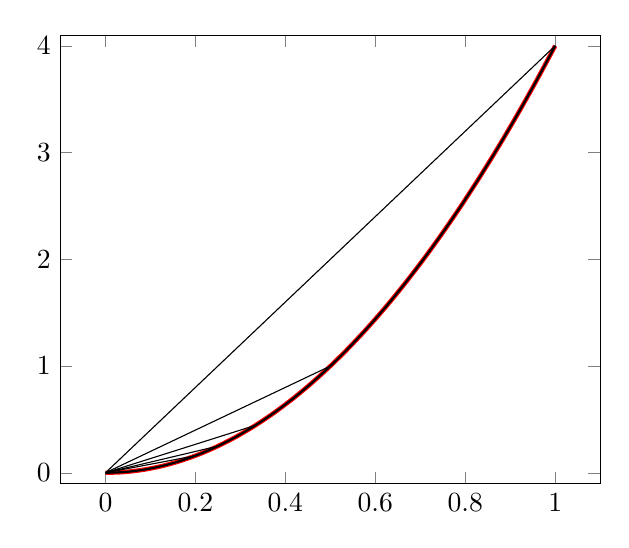
\begin{tikzpicture}
        \begin{axis}[ymin=-0.1, ymax=4.1, xmin=-0.1, xmax=1.1]
          \addplot[smooth,color=red,ultra thick,domain=0:1]{(2*x)^2};
          \foreach \n in {1,...,5}
          {
            \addplot[smooth,domain=0:(1/(\n))]{\n*x*(2/\n)^2};
          }
          \addplot[smooth,color=black,thick,domain=0:1]{(2*x)^2};
        \end{axis}
      \end{tikzpicture}
      \caption{ Een illustratie van de situatie voor $f(x) = x^{2}$}
    \end{figure}
    \end{itemize}
  \end{proof}
\end{vb}


\subsection{De $d_2$-metriek op $C(\interval{0}{1})$}
\label{sec:de-d_2-metriek}

\begin{vb}
  Zij $\interval{a}{b}$ een gesloten begrensd interval, dan is $C(\interval{a}{b})$, uitgerust met de volgende functie als metriek, een metrische ruimte:
  \[ d_{2}:\ C(\interval{a}{b})\times C(\interval{a}{b}) \rightarrow \mathbb{R}^{+}:\ (f,g) \mapsto \sqrt{\int_{a}^{b}|f(x)-g(x)|dx} \]
  \extra{bewijs}
  Hint uit de les: het bewijs reduceert zich tot dit:
  \[ \left|\int_{a}^{b}f(x)g(x)\right| < \left(\int_{a}^{b}f(x)^{2}\ dx \right) \left(\int_{a}^{b}g(x)^{2}\ dx \right) \]
  Los hiervoor volgende ongelijkheid uit de genormeerde vectorruimte op met een discriminant.
  \[ \left\| v+\lambda w \right\| > 0 \]
\end{vb}

\begin{st}
  $\forall f,g \in C(\interval{a}{b}):\ d_{1}(f,g) \le d_{\infty}(f,g)$
\extra{bewijs}
\end{st}

\begin{de}
  Noem de verzameling functies $f:\ \mathbb{R} \rightarrow \mathbb{R}$ die in beide oneindigheden naar $0$ gaan: $C_{0}(\mathbb{R})$.
\end{de}

\begin{vb}
  De functie $d$ als volgt, is niet alleen geen metriek voor $C_{0}(\mathbb{R})$, ze is ook niet goed gedefinieerd.
  \[ \int_{-\infty}^{+\infty}|f(x)-g(x)|\ dx \]
  De integraal bestaat immers niet steeds.
\end{vb}

\begin{vb}
  De functie $d$ als volgt, is een metriek voor $C_{0}(\mathbb{R})$.
  \[ d(f,g) = \int_{-\infty}^{+\infty}\frac{|f(x)-g(x)|}{1+x^{2}}\ dx \]
 \extra{bewijs}
\end{vb}

\subsection{Andere metrieken op $C(\interval{0}{1})$}
\label{sec:andere-metrieken-op}

\begin{vb}
  Zij $D$ een deelverzameling van $Q \cap \interval{0}{1}$.
  De functie $d_{D}$ als volgt is een metriek op $C(\interval{0}{1})$.
  \[ d_{D}:\ C(\interval{0}{1})^{2} \rightarrow \mathbb{R}:\ d_{D}(f,g) = \sum_{k=1}^{\infty}\frac{1}{2^{k}}\left| f(x_{k}) - g(x_{k})\right| \]
  Hierin zijn de elementen van $D$ (in om het even welke volgorde) genummerd.
  
  \begin{proof}
    Eerst is het belangrijk op te merken dat $d_{D}$ goed gedefinieerd is.
    De functies in $C(\interval{0}{1})$ zijn immers begrensd.\stref{st:gesloten-en-begrensd-interval-continu-dan-uniform-continu}\prref{pr:uniform-continu-beeld-van-begrensd-deel-begrensd}
    \begin{itemize}
    \item De symmetrie van $d_{D}$ is evident vanuit de definitie.
    \item De tweede eigenschap van een metriek is niet even evident.
      We zullen goed moeten gebruiken dat $D$ dicht ligt in $\interval{0}{1}$.
      Stel nu dat er tussen twee functies $f$ en $g$ een $d_{D}$ afstand nul is, maar ze toch niet gelijk zijn.
      We leiden dan een contradictie af met de continuiteit van $f$ of $g$.
      Omdat de afstand tussen $f$ en $g$ nul is, zijn $f$ en $g$ al gelijk in alle punten $x_{k}$.
      Omdat $f$ en $g$ niet gelijk zijn, bestaat er een punt $y\in \interval{0}{1} \setminus D$ waarin $f$ en $g$ verschillen.
      Omdat $D$ dicht ligt in $\interval{0}{1}$, bestaat er dus een rij $(x_{k_{n}})_{n}$ in $D$ die naar $y$ convergeert.
      Omdat $(f-g)$ nul is in elk punt $x_{k_{n}}$ zal de rij $((f-g)(x_{k_{n}}))_{n}$ dus niet naar het verschil tussen $f$ en $g$ in $y$ convergeren maar naar $0$.
      Dit betekent dat $(f-g)$ niet continu\prref{pr:continu-asa-behoudt-convergentie} en dus ofwel $f$ ofwel $g$ niet continu.\prref{pr:optelling-continu}
    \item De driehoeksongelijkheid:
      \begin{align*}
        d(f,g)
        &= \sum_{k}\frac{1}{2^{k}}\left| f(x_{k}) - g(x_{k})\right|\\
        &= \sum_{k}\frac{1}{2^{k}}\left| f(x_{k}) - h(x_{k}) + h(x_{k}) - g(x_{k})\right|\\
        &\le \sum_{k}\frac{1}{2^{k}}\left| f(x_{k}) - h(x_{k})| + |h(x_{k}) - g(x_{k})\right|\\
        &= d(f,h) + d(h,g)
      \end{align*}
    \end{itemize}
  \end{proof}
\end{vb}

\begin{tvb}
  Als $D$ hierboven verzameling zou zijn die niet dicht is in $\interval{0}{1}$, dan is $d_{D}$ geen metriek.

  \begin{proof}
    We construeren twee functies $f,g \in \interval{0}{1}$ op $d_{D}$ afstand $0$ die niet gelijk zijn.
    Omdat $D$ niet dicht ligt in $\interval{0}{1}$, bestaat er een punt $x\in \interval{0}{1}$ dat niet in de sluiting van $D$ ligt.\deref{de:dicht-liggen}
    Laat $f$ en $g$ gelijk zijn in alle punten van $D$ en op een continue manier verschillen in $x$.

    \noindent Nog concreter:\\
    Kies $D = \{ \left(\frac{1}{n}\right) \mid n\in\mathbb{N} \}$ en $f$ en $g$ als volgt:

    \noindent
    \begin{minipage}{.45\textwidth}
      \begin{figure}[H]
        \centering
        \begin{tikzpicture}[scale=.75]
          \begin{axis}[ymin=-1.1, ymax=1.1, xmin=-0.1, xmax=1.1]
            \addplot[smooth,color=blue,thick,domain=0:1/2]{0};
            \addplot[smooth,color=red,thick,domain=0:1/2]{0};
            \addplot[smooth,color=blue,thick,domain=1/2:3/4]{x-1/2)};
            \addplot[smooth,color=red,thick,domain=1/2:3/4]{-x+1/2)};
            \addplot[smooth,color=blue,thick,domain=3/4:1]{-x+1)};
            \addplot[smooth,color=red,thick,domain=3/4:1]{(x-1)};
            \foreach \i in {1,...,100}{
              \addplot[soldot,color=green,thin] coordinates{(1/\i,0)};
            }
          \end{axis}
        \end{tikzpicture}
      \end{figure}
    \end{minipage}
    \begin{minipage}{.45\textwidth}

      \begin{align*}
        f(x) = 
        \begin{cases}
          0 &\text{ als } x \in \interval{0}{\frac{1}{2}}\\
          \left(x-\frac{1}{2}\right) &\text{ als } x \in \interval[open]{\frac{1}{2}}{\frac{3}{4}}\\
          -\left(x-\frac{1}{2}\right) &\text{ als } x \in \interval{\frac{3}{4}}{1}
        \end{cases}\\
        g(x) = 
        \begin{cases}
          0 &\text{ als } x \in \interval{0}{\frac{1}{2}}\\
          -\left(x-\frac{1}{2}\right) &\text{ als } x \in \interval[open]{\frac{1}{2}}{\frac{3}{4}}\\
          \left(x-\frac{1}{2}\right) &\text{ als } x \in \interval{\frac{3}{4}}{1}
        \end{cases}\\
      \end{align*}
    \end{minipage}
  \end{proof}
\end{tvb}


\end{document}

%%% Local Variables:
%%% mode: latex
%%% TeX-master: t
%%% End:
